\chapter{MongoDB (Fabian)}\label{mongodb-fabian}

\section{Einleitung}\label{einleitung}

\begin{figure}[h]
	\centering
	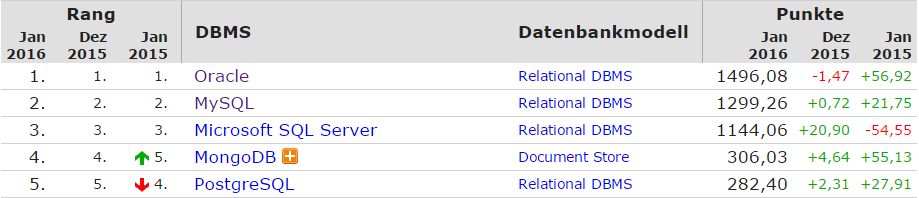
\includegraphics[width=0.7\linewidth]{figures/db-ranking.png}
	\caption{Datenbanken Ranking Datenquelle: db-engines \cite{db-engines:mongodb}}
	\label{f:mongodb:ranking}
\end{figure}

Die Entwicklung von MongoDB wurde im Jahr 2007 von dem Unternehmen 10gen
ins Leben gerufen. Hierfür wurde die Programmiersprache C++ verwendet.
Da die Datenmengen durch Big Data heutzutage rasant steigen
werden die Skalierbarkeit und die Performanz bei großen Datenmengen zu
immer wichtigeren Themen. MongoDB wirbt mit agility, scalability und
performance. Dies soll durch denn Einsatz von verteilten Systemen
ermöglicht werden. Der Name mongo leitet sich aus dem Wort humongous ab,
welches gigantisch bedeutet. Hierdurch wird auf die Idee eine Datenbank
für große Datenmengen zu entwickeln angespielt.

Wie in der Abbildung \ref{f:mongodb:ranking} zu sehen steht MongoDB aktuell auf dem
vierten Platz der populärsten Datenbanken. Damit ist sie hinter drei
klassischen Relational Database Management System (RDBMS) die populärste
NoSQL-Datenbank.

\section{Konzepte}\label{konzepte}

Eine herkömmliche RDBMS besteht aus Datenbanktabellen, die einem festen
Schema unterliegen. Bei MongoDB dagegen handelt es sich um eine
Schema-freie, dokumentenbasierte Open-Source-Datenbank. Diese beinhaltet
Sammlungen, die jeweils aus mehreren Dokumente ohne ein festes Schema
bestehen. Jedes Dokument darin kann sich von den Feldern und Strukturen
von den anderen unterscheiden. Dokumente bestehen aus mehreren
Schlüsselwert-Paaren und stellen die Basiseinheit für Daten dar. Die
hierbei verwendbaren Datentypen sind die bekannten Standard-Datentypen
(Integer, Float, Boolean, String, Array), Date, Embedded-Doc, DBRef und
ObjectID. Es gibt unterschiedliche Wege in der Datenbank zu
referenzieren. Dies kann durch Verschachtelung der Dokumente geschehen.
Allerdings führt dies zu einer hohen Komplexität, wenn ein update auf
eine verschachtelte Information durchgeführt werden soll. Bei der
ObjectID handelt es sich um die Standard ID, die jedes Dokument
aufweist. Diese wird bei der Erzeugung eines jeden Dokuments generiert
und ist durch ihren komplexen Aufbau eindeutig. Durch Verwendung der
ObjectID können auch Referenzen hergestellt werden. Bei Verwendung von
ObjectID handelt es sich im Gegensatz zu verschachtelten Dokumenten um
einen ``echten'' Join. Der DBRef entspricht dem Fremdschlüssel aus dem
RDBMS. Also dient er als Identifier für Dokument / Collection /
Datenbank. MongoDB verwendet eine integrierte Query Language. Durch
diese können die Create, Read, Update, Delete (CRUD) Operationen
realisiert werden.

Die Replikationen spielen bei NoSQL-Datenbanken eine zentrale Rolle. Die
Replikationen bestimmen über die Synchronisierung von Daten über mehrere
Server. Bei MongoDB funktionieren diese nach dem Master-Slave-Prinzip.
D.h. es existiert ein Replikationsset. Dieses besteht aus einem primären
und beliebig vielen sekundären Knoten. Alle Schreiboperationen gehen nur
an den primären Knoten. Dieser synchronisiert seine sekundären Knoten
erst nach und nach. Das bedeutet, dass die Daten für eine gewisse Zeit
inkonsistent sind. Es kann daher keine Konsistenz zum
Transaktionszeitpunkt garantiert werden wie bei RDBMS. Im schlimmsten
Fall funktioniert die Schreiboperation auf den primären Knoten und
dieser fällt bevor er die Schreiboperation an die sekundären Knoten
weitergegeben hat aus. Dies führt nämlich zu Datenverlust, MongoDB denkt
aber die Operation wurde erfolgreich durchgeführt. Ein Vorteil ist, dass
ein automatischer failover möglich ist. Falls also der primäre Knoten
nicht erreicht werden kann wird ein ehemals sekundärer Knoten zum neuen
primären. Bei Leseoperationen dagegen kann auch auf die sekundären
Knoten zugegriffen werden, um einen Skalierungseffekt zu erhalten. Einen
Flaschenhals stellen also die Schreiboperationen dar, die
Leseoperationen eher nicht. Dies birgt allerdings das Risiko alte
Datenstände zurückzubekommen. Der daraus resultierende erhöhte
Speicherbedarf fällt dank dem Einsatz verteilter Systeme nicht ins
Gewicht. Allerdings sorgen die Replikationen für eine hohe Verfügbarkeit
und dienen auch als Backup der Daten.

Um denn in der heutigen Zeit nicht ungewöhnlichen wachsenden Datenmengen
zu begegnen gibt es automatisches Sharding. Dieses sorgt für die
Verteilung der Daten über mehrere Systeme. Dies wird auch als
horizontale Skalierung bezeichnet. Dies bietet vielfältige Vorteile. Zum
einen verursacht das vertikales Skalieren, also der Einsatz immer
besserer Hardware exponentielle Kosten. Zum anderenen ist der Lokale
Speicher möglicherweise einfach nicht groß genug. Die Komponenten sind
Shards, Config Server und mongos. Jedes Shard entspricht einem oben
beschriebenen Replikationsset. Die Config Server beinhalten die
Metadaten von dem Cluster. Sprich eine Map von den angefragten Daten und
wo sie gespeichert sind. Um Redundanz und Verfügbarkeit zu gewährleisten
muss es drei Config Server geben. Dann gibt es noch die mongos. Diese
werden von der Applikation angesprochen und führen die query Kommandos
aus.

Die Daten werden im sogenannten BSON Format gespeichert und
ausgetauscht.

Bedingt durch die oben genannten Konzepte ist eine strenge Einhaltung der ACID (atomar, consistency, isolation, durability) Kriterien nicht möglich. Es wird ein Tradeoff von Konsistenz und Isolation zu einer besseren Performanz und Skalierbarkeit eingegangen. Da man auf Konsistenz allerdings nicht vollständig verzichten kann wird das abgeschwächte BASE (Basically Available, Soft state, Eventual consistency) angestrebt. Hierbei wird nur eine "weiche" Konsistenz gewährleistet. Dadurch steigt der Aufwand für die Anwendungsentwicklung, die daraus entstehende Probleme abfangen muss.

\section{Usecases}\label{usecases}

\begin{itemize}
\itemsep1pt\parskip0pt\parsep0pt
\item
  rapid prototyping
\item
  Leselastige Anwendungen
\end{itemize}

\section{Mongoose}\label{mongoose}

Bei Mongoose handelt es sich um eine Bibliothek für das Node Framework. Durch diese Bibliothek soll Object Data Modelling (ODM) im Zusammenhang mit MongoDB als Datenbank ermöglicht werden.

Der Hauptvorteil von Mongoose besteht in der Abstraktion von Daten der MongoDB. Viele Entwickler, die es vorher mit SQL-Datenbanken zu tun hatten dürften damit wesentlich besser zurecht kommen, als mit den dynamischen Sammlungen von MongoDB. Durch das Verwenden von Schemas und Models können Strukturen definiert werden.

Außerdem bietet diese Bibliothek auch noch einige andere Funktionalitäten. Unter anderem zum Einsatz von Middleware, Plug-Ins und zur Validierung.

Mongoose verwendet das Konzept Active Records. Dies ist ein durchaus umstrittenes Konzept, da es auf der einen Seite als leicht und schnell erlernbar gesehen wird, allerdings auf der anderen Seite das Testen erschwert und zu Flaschenhälsen in der Performanz führt.

Die Dokumentation auf der offiziellen Webseite ist sehr unübersichtlich. Hierdurch wird das Arbeiten mit dieser Bibliothek erschwert.

Die aktuelle Version von Mongoose wurde im Januar 2016 als 4.3.5. veröffentlicht.
